\documentclass[nooutcomes]{ximera}
\usepackage{fullpage}
%% handout
%% space
%% newpage
%% numbers
%% nooutcomes


\newcommand{\RR}{\mathbb R}
\renewcommand{\d}{\,d}
\newcommand{\dd}[2][]{\frac{d #1}{d #2}}
\renewcommand{\l}{\ell}
\newcommand{\ddx}{\frac{d}{dx}}
\newcommand{\dfn}{\textbf}
\newcommand{\eval}[1]{\bigg[ #1 \bigg]}

\usepackage{multicol}

\renewenvironment{freeResponse}{
\ifhandout\setbox0\vbox\bgroup\else
\begin{trivlist}\item[\hskip \labelsep\bfseries Solution:\hspace{2ex}]
\fi}
{\ifhandout\egroup\else
\end{trivlist}
\fi}

\title{4.4: Optimization}

\begin{document}
\begin{abstract}
\end{abstract}
\maketitle

%problem 1
\begin{problem}

  Suppose you want to maximize a continuous function on a closed interval, but you find that it only has one local extremum on the  interval which happens to be a local minimum.
  Where else should you check for the solution?
\begin{freeResponse}
  The endpoints.
\end{freeResponse}	
\end{problem}

%problem 2
\begin{problem}
Find the radius of a cylindrical container with a volume of $2 \pi\ m^3$ that minimizes the surface area.


  \begin{image}
    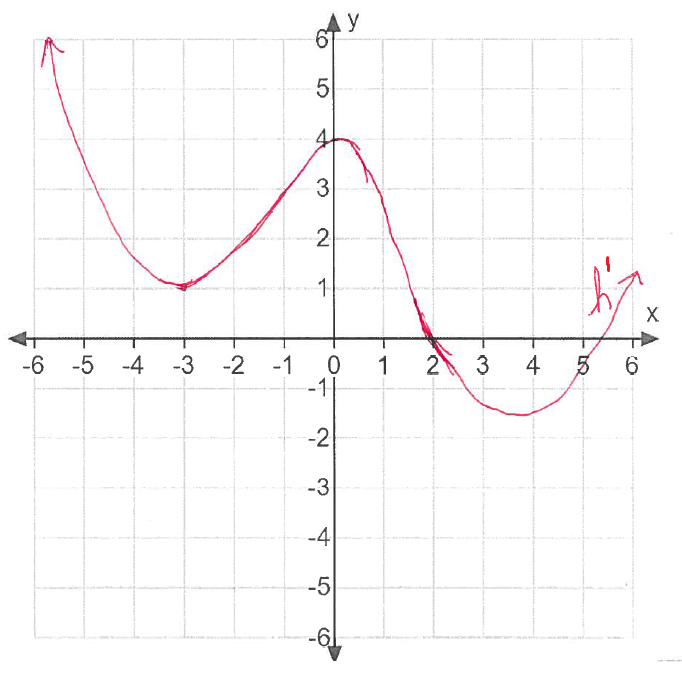
\includegraphics[scale = 0.6]{Images/figure1.png}
  \end{image}

\begin{freeResponse}

We have two formulas: $V=\pi r^2h$ and $S=2 \pi rh+2r^2\pi$.  We know $V=2\pi$ and want to find the $r$ that minimizes $S$.  Since we need a forumula for $S$ only in terms of $r$ we are going to rewrite $V=\pi r^2h$ to give us a formula for for $h$ in terms of $r$.

\begin{align*}
V=2\pi \text{and}\ V=\pi r^2h \implies 2\pi &= \pi r^2h\\
\frac{2\pi}{\pi r^2}&=h\\
\frac{2}{r^2}&=h\\
\implies S(r)&=2 \pi r\left(\frac{2}{r^2}\right)+2r^2\pi\\
S(r)&=\frac{4\pi}{r}+2r^2\pi
\end{align*}

The domain is $(0,\infty)$.

Next, we need to minimize $S$.
\begin{align*}
S'(r)&=\frac{-4\pi}{r^2}+4\pi r\\
&=4\pi \left(r-\frac{1}{r^2}\right)
\end{align*}

To find the critical points:
\begin{align*}
r-\frac{1}{r^2}&=0\\
r&=\frac{1}{r^2}\\
r^3&=1\\
r&=1
\end{align*}

The only critical point of $S$ is at $r=1$.  We need to verify $r=1$ is a minimum.

We can use the second derivative test:
\begin{align*}
S''(r)&=8\pi r^{-3}+4\pi\\
\implies S''(1)&=8\pi+4\pi>0
\end{align*}

The function $S$ has a local minimum at $r=1$.  So $(1,S(1)$ is the absolute minimum since this is the only critical point.  (See Theorem 4.5).


\end{freeResponse}

\end{problem}

%problem 3
\begin{problem}

  A part of a circle centered at the origin with radius $r = 7 \text{ cm}$ is given in the figure (A) below.
  A right triangle is formed in the first quadrant (see figure (A)).
  One of its sides lies on the $x$-axis.
  Its hypotenuse runs from the origin to a point on the circle.
  The hypotenuse makes an angle $\theta$ with the $x$-axis.

  \begin{image}
    \includegraphics[scale = 0.2]{Images/"maximize triangle in circle".png}
    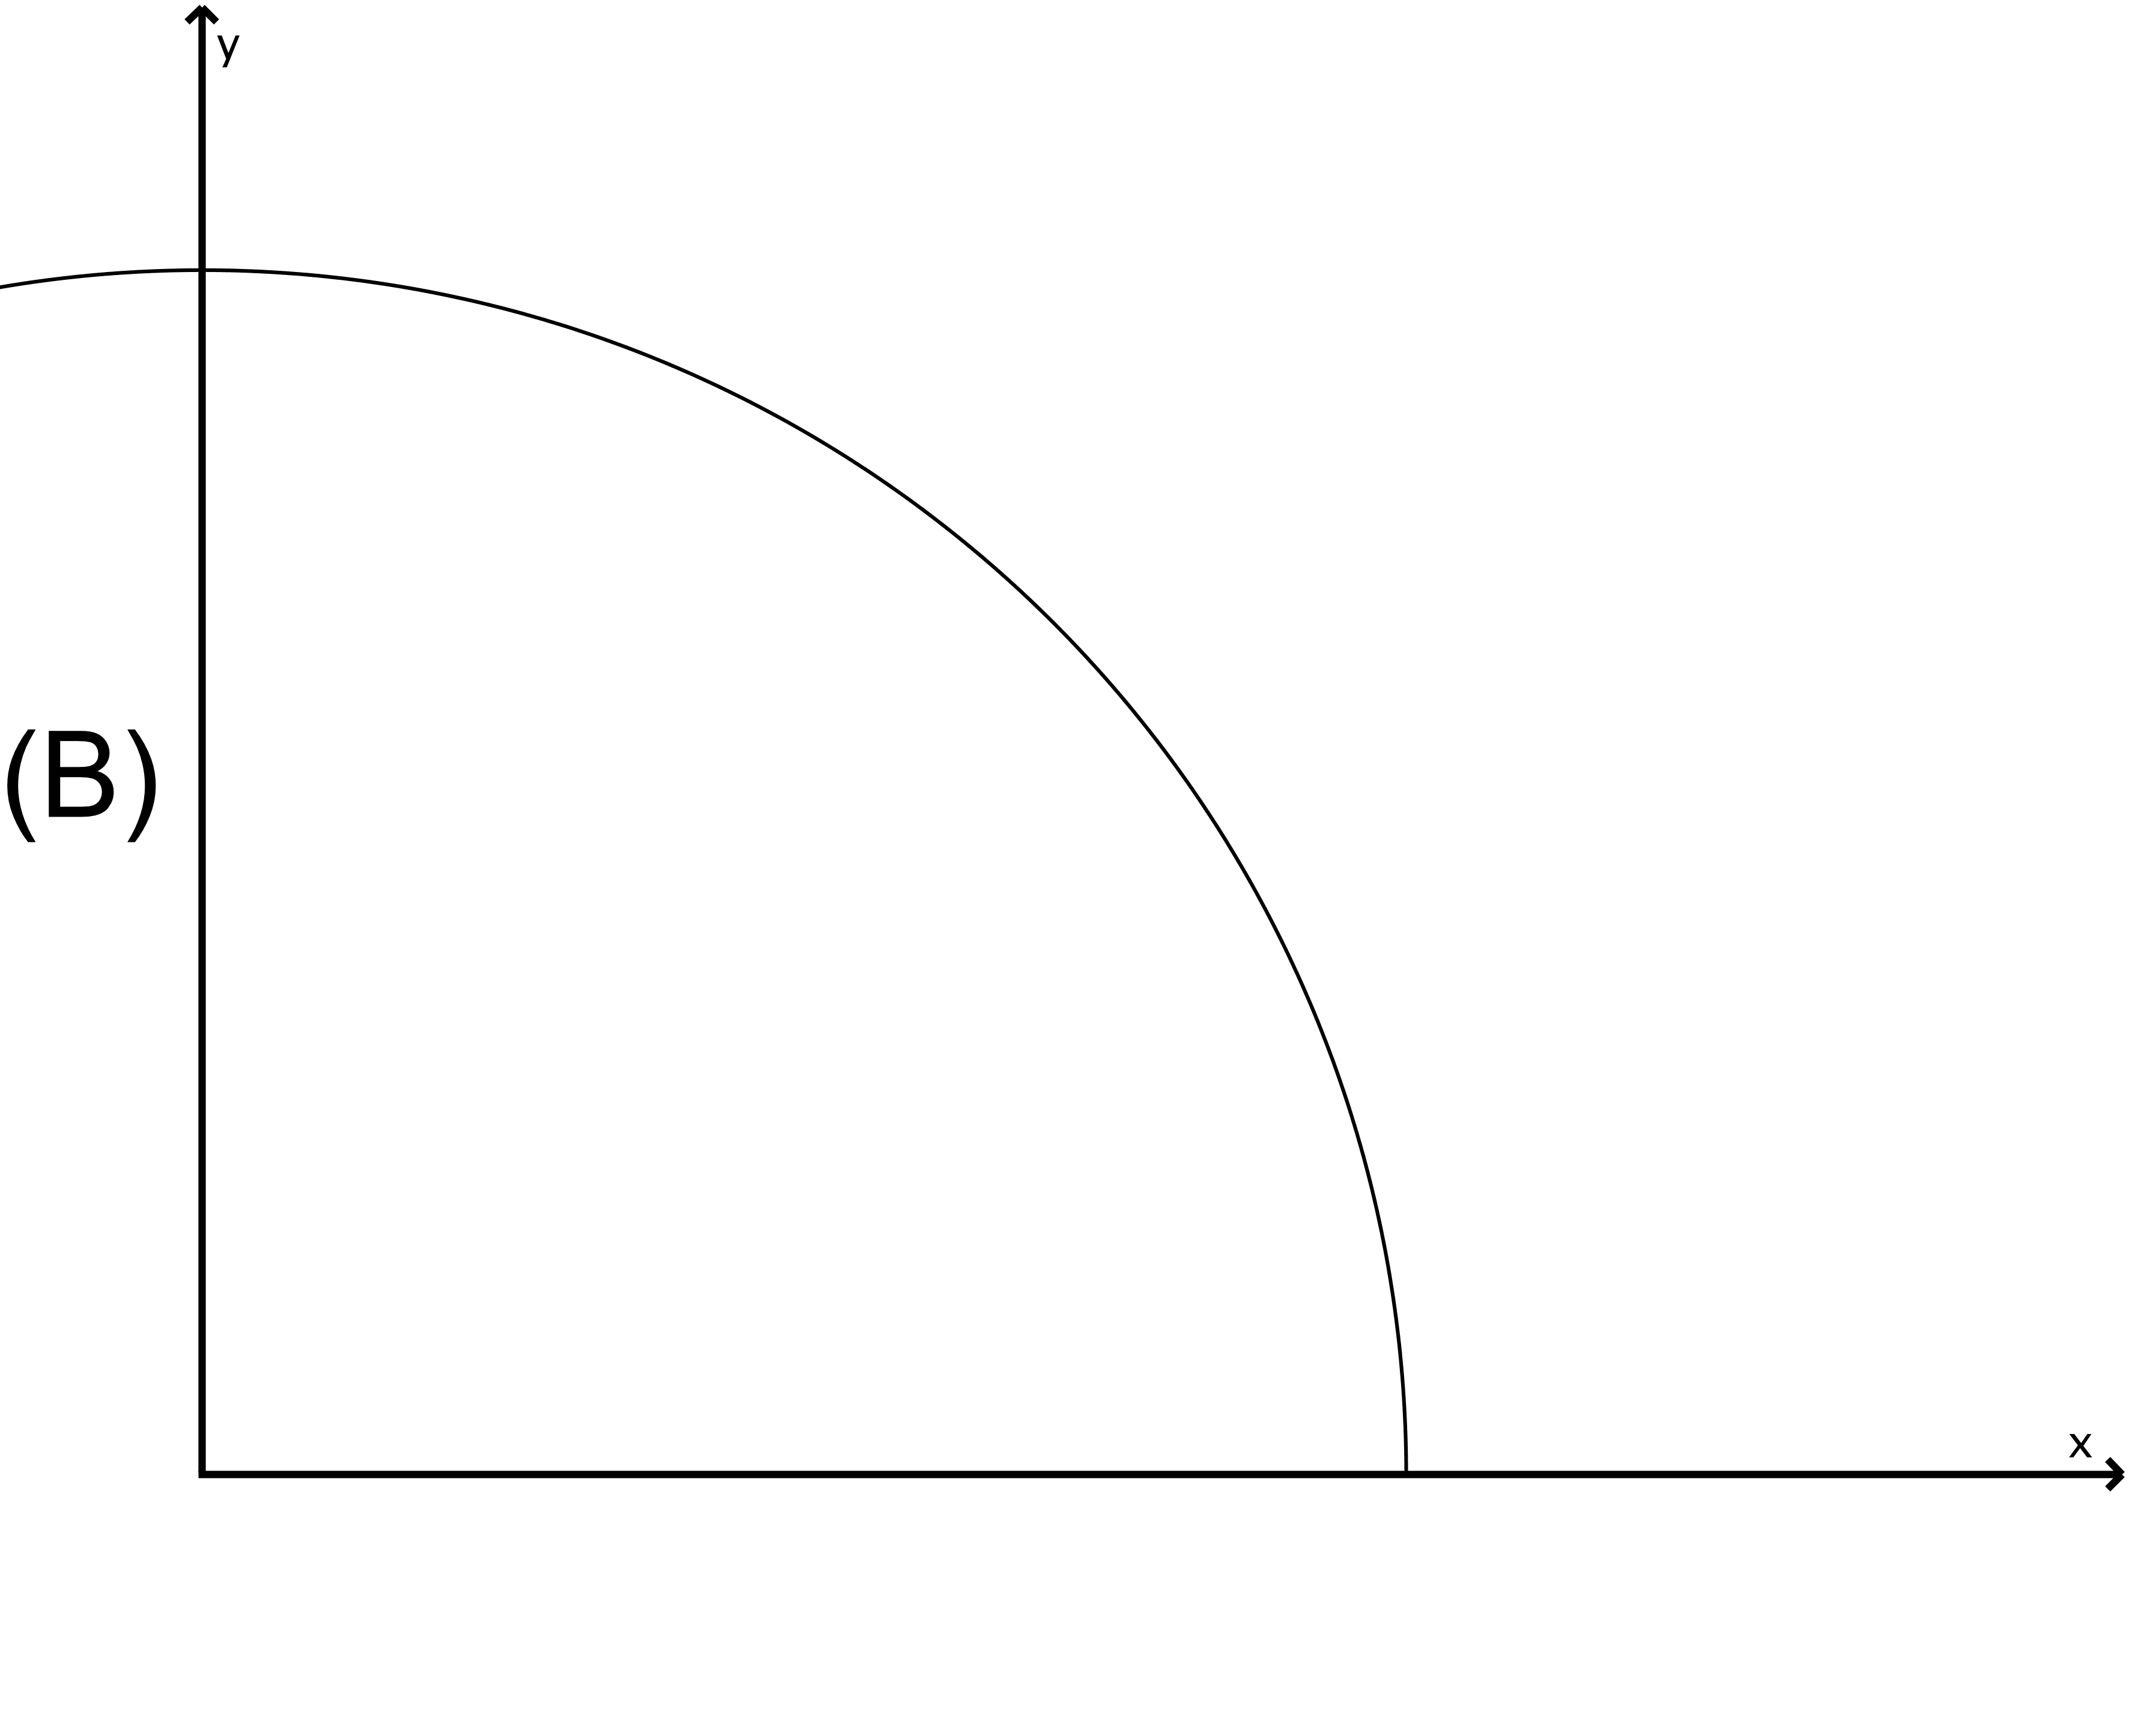
\includegraphics[scale = 0.2]{Images/figure7.png}
  \end{image}
  Make sure to label the picture.

  \begin{enumerate}
    \item
      Draw 2 more examples of such a triangle in the figure (B).
      \begin{freeResponse} \hfil
      
  \begin{image}
    \includegraphics[scale = 0.15]{Images/"Two more triangles".png}
      \end{image}
 
      \end{freeResponse}

    \item
      Express the area of such a triangle as a function of $\theta$ and state its domain.
      \begin{freeResponse}
        The area of a triangle is $(1/2)\cdot\mbox{ base } \cdot \mbox{ height }$.
        The base of the triangle is $7\cos(\theta)$ and the height is $7\sin(\theta)$.

        Therefore:
        \begin{align*}
          A(\theta) &= \frac{1}{2}\cdot 7\cos(\theta) \cdot 7\sin(\theta)\\
                    &= \frac{49}{2}\cos(\theta)\sin(\theta)
        \end{align*}

        and
        \begin{align*}
          \mbox{Domain of $A$ = $[0,\pi/2]$}
        \end{align*}
      \end{freeResponse}

    \item
      Find the value of $\theta$ which maximizes the area in part (b).
      Show your work and justify your answer.
      \begin{freeResponse}
        Finding critical points:
        \begin{align*}
          A'(\theta) &= \frac{-49}{2} \sin(\theta)\sin(\theta) + \frac{49}{2}\cos(\theta)\cos(\theta) \\
          &\implies A'(\theta) = 0\\
          &\implies \cos^2(\theta) = \sin^2(\theta)\\
          &\implies \cos(\theta) = \sin(\theta)\\
          &\implies \theta = \frac{\pi}{4}
        \end{align*}

        Locating absolute maximum:
        \begin{align*}
          A(0) = 0, A(\pi/4) = \frac{49}{4}, A(\pi/2) = 0 &\implies \mbox{absolute maximum at $\theta = \pi/4$}
        \end{align*}
      \end{freeResponse}
  \end{enumerate}
\end{problem}

%problem 4
\begin{problem}
  A cone is constructed by cutting a sector from a circular sheet of metal with radius 20.
  The cut sheet is then folded and welded.
  Find the radius and height of the cone with maximum volume that can be formed this way.

  \begin{image}
    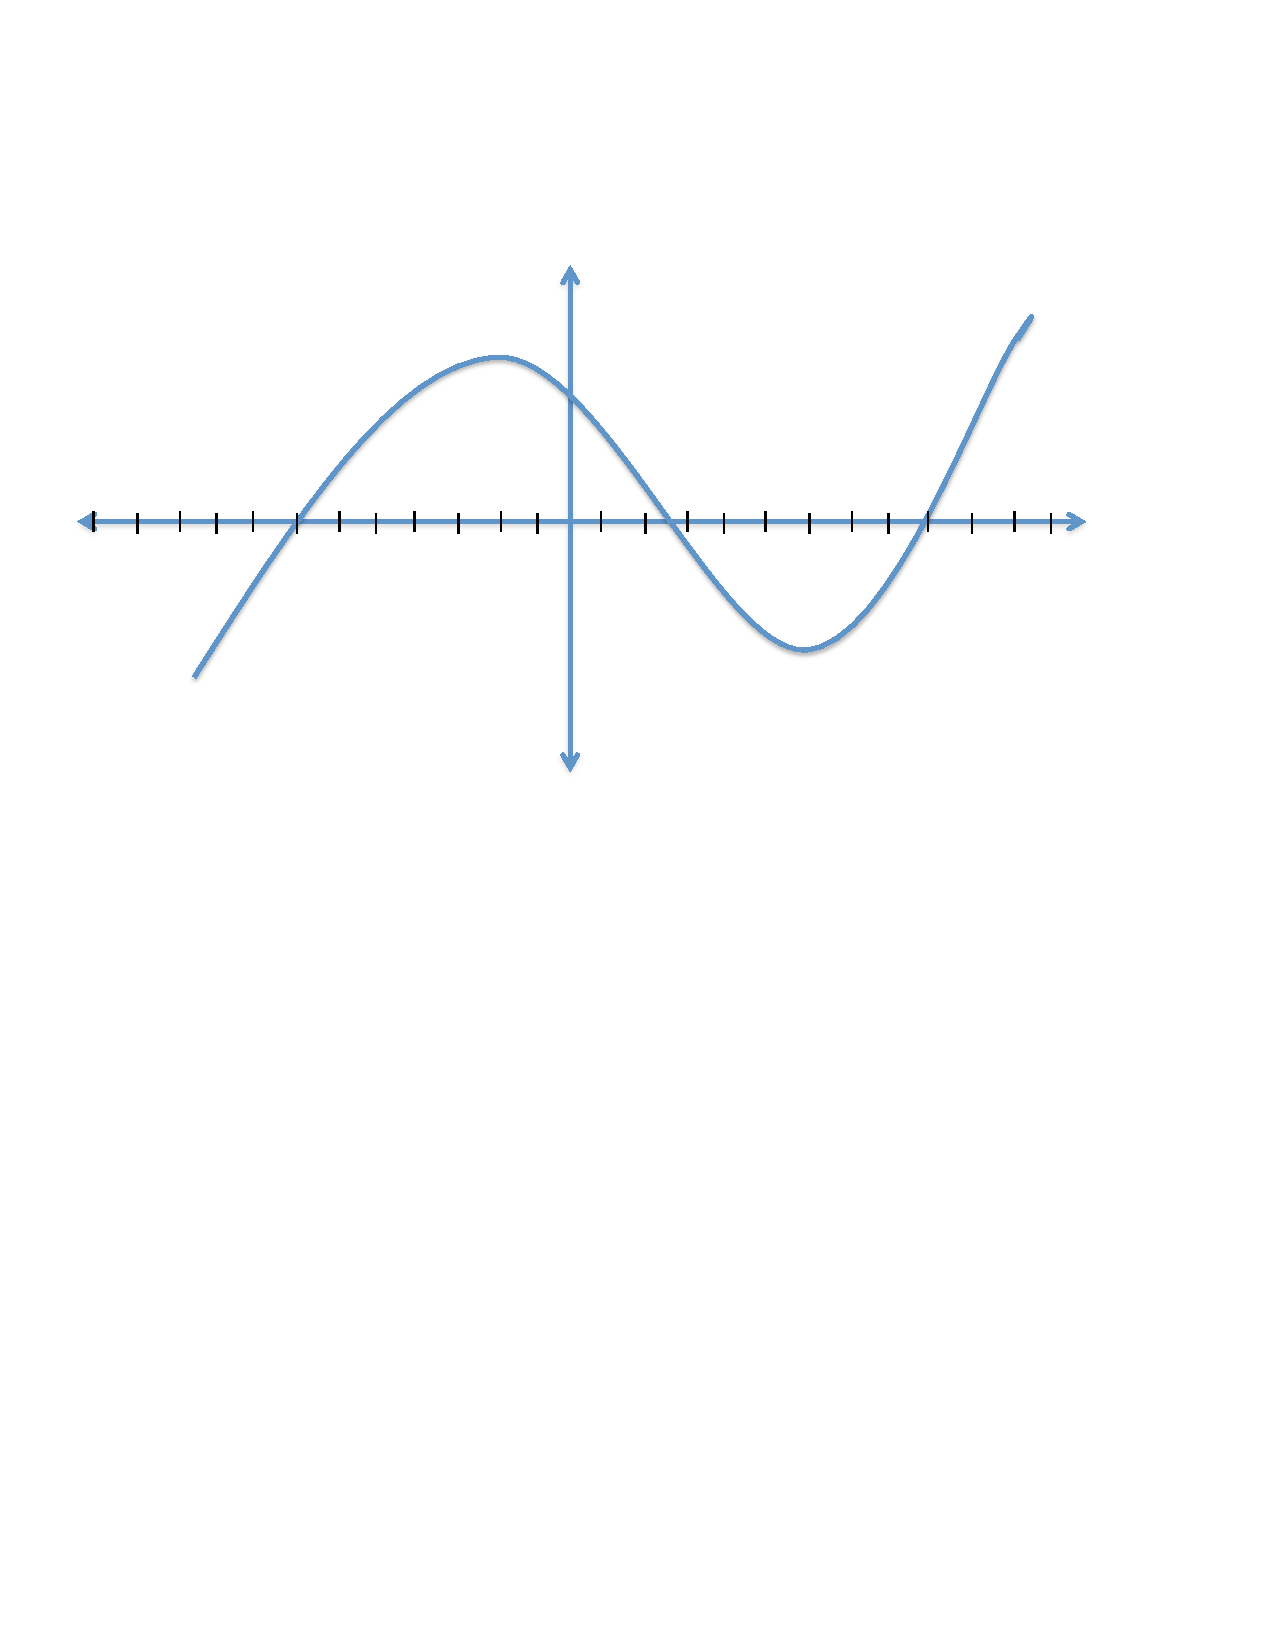
\includegraphics[trim= 100 530 250 190]{Images/Figure2.pdf}
  \end{image}
	
  \begin{freeResponse}
    First, recall that the volume of a cone is
    \begin{equation}
      \label{cone volume}
      V = \frac{1}{3} \pi r^2 h
    \end{equation}
		
    Equation \eqref{cone volume} has two variables, $r$ and $h$.  
    So we need to find a constraint equation.  
    Notice that the length of the cone is a fixed length of 20.  
    So using Pythagorean's Theorem we have that:
    \begin{equation}
      \label{constraint}
      r^2 + h^2 = 20^2 = 400
    \end{equation}
		
    Solving equation \eqref{constraint} for $r^2$, we get $r^2 = 400 - h^2$.  
    Plugging this into equation \eqref{cone volume} gives
    \begin{equation}
      \label{V(h)}
      V = \frac{1}{3} \pi (400-h^2) h = \frac{1}{3} \pi (400h - h^3) 
    \end{equation}
    Note that, due to the settings of the problem, the domain for $h$ is $[0,20]$.  
		
    It is worth pointing out that it is a lot easier algebraically to solve for $r^2$ in equation \eqref{constraint} and then plug into equation \eqref{cone volume} instead of doing the same thing for $h$.

    Now we need to differentiate equation \eqref{V(h)} with respect to $h$, set this equal to $0$, and solve for $h$.
    $$ \dd[V]{h} = \frac{1}{3} \pi (400 - 3h^2) := 0 $$
    $$ 400 - 3h^2 = 0 $$
    $$ 3h^2 = 400 $$
    $$ h^2 = \frac{400}{3} $$
    $$ h = \pm \sqrt{\frac{400}{3}} = \pm \frac{20}{\sqrt{3}} $$
    but $- \frac{20}{\sqrt{3}}$ is not in our domain for $h$, and so the only critical point for $V(h)$ is $h = \frac{20}{\sqrt{3}}$.  
    We need to show that this is an absolute maximum for $V(h)$ on $[0,20]$.  
    Since $[0,20]$ is a closed interval, we can just evaluate $V(h)$ at $h=0, \frac{20}{\sqrt{3}}, 20$.  
    \begin{align}
      V(0) &= \frac{1}{3} \pi (0-0) = 0 \\
      V \left( \frac{20}{\sqrt{3}} \right) &= \frac{1}{3} \pi \left( \frac{20^3}{\sqrt{3}} - \frac{20^3}{\left( \sqrt{3} \right)^3} \right) > 0 \label{inequality} \\
      V(20) &= \frac{1}{3} \pi (20^3 - 20^3) = 0 
    \end{align}
		
    Thus $h=\frac{20}{\sqrt{3}}$ maximizes the volume of the cone.
    Then $$r^2 = 400 - h^2 = 400 - \left( \frac{20}{\sqrt{3}} \right)^2 = 400 - \frac{400}{3} = \frac{800}{3}$$ and so $$ r = 20 \sqrt{\frac{2}{3}}. $$
		
    If you are not comfortable with inequality \eqref{inequality} above without a calculator, then a nice alternative is to use the second derivative test instead to check that $h=\frac{20}{\sqrt{3}}$ maximizes the volume of the cone.
    This works since this is the only critical point in the domain of $h$.
    To do this, compute
    $$ \dd[^2V]{h^2} = \frac{1}{3} \pi (-6h) $$
    $$ \eval{\dd[^2V]{h^2}}_{h=\frac{20}{\sqrt{3}}} = \frac{1}{3} \pi \left( -6 \left(\frac{20}{\sqrt{3}} \right) \right) < 0 $$
    and thus this value for $h$ gives a local (and therefore, absolute) maximum value for $V(h)$.  
  \end{freeResponse}
\end{problem}

%problem 5
\begin{problem}

  A rectangular flower garden with an area of $30 \, m^2$ is surrounded by a grass border $1 \, m$ wide on two sides and $2 \, m$ wide on the other two sides (see figure).
  What dimensions of the garden minimize the combined area of the garden and borders?
  
  \begin{image}
    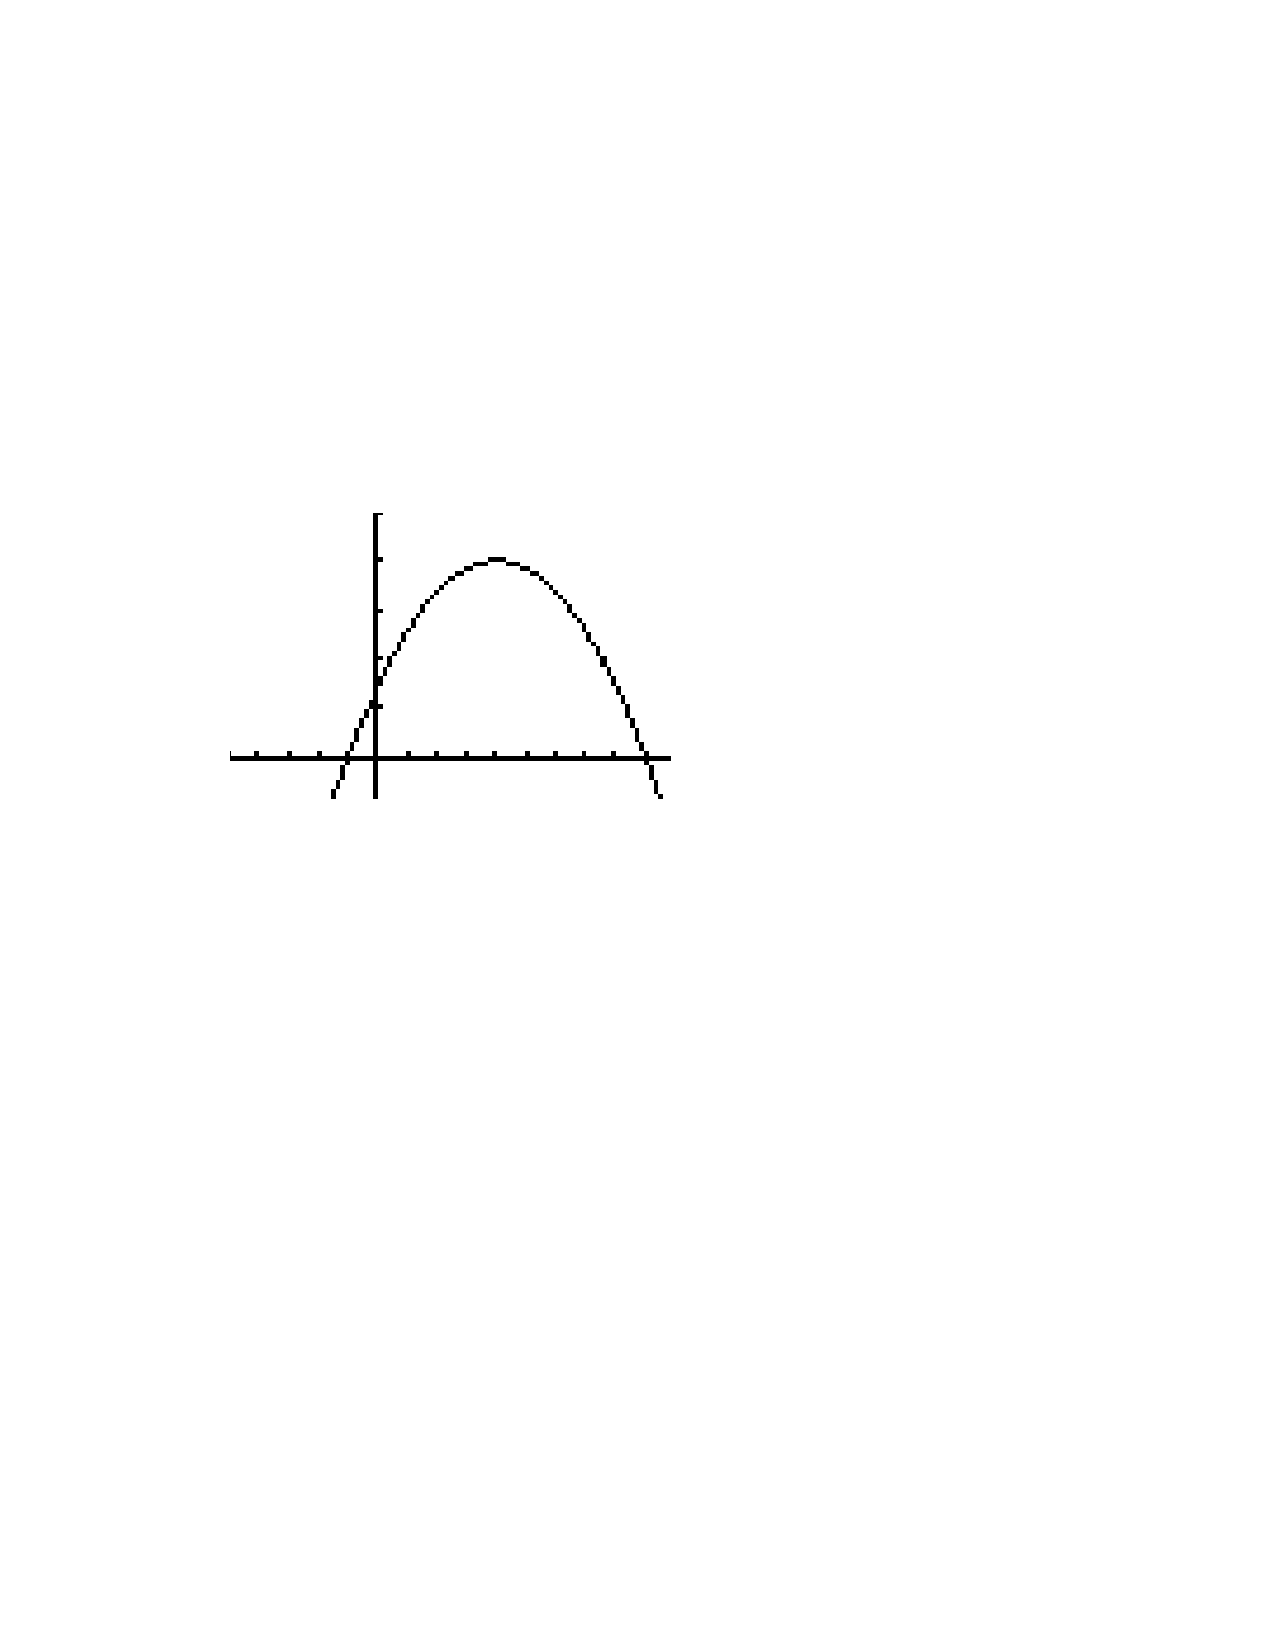
\includegraphics[trim= 100 480 250 250]{Images/Figure1.pdf}
  \end{image}

  \begin{enumerate}
    \item  Label the picture with variables.
      \begin{freeResponse}
        \begin{image}
          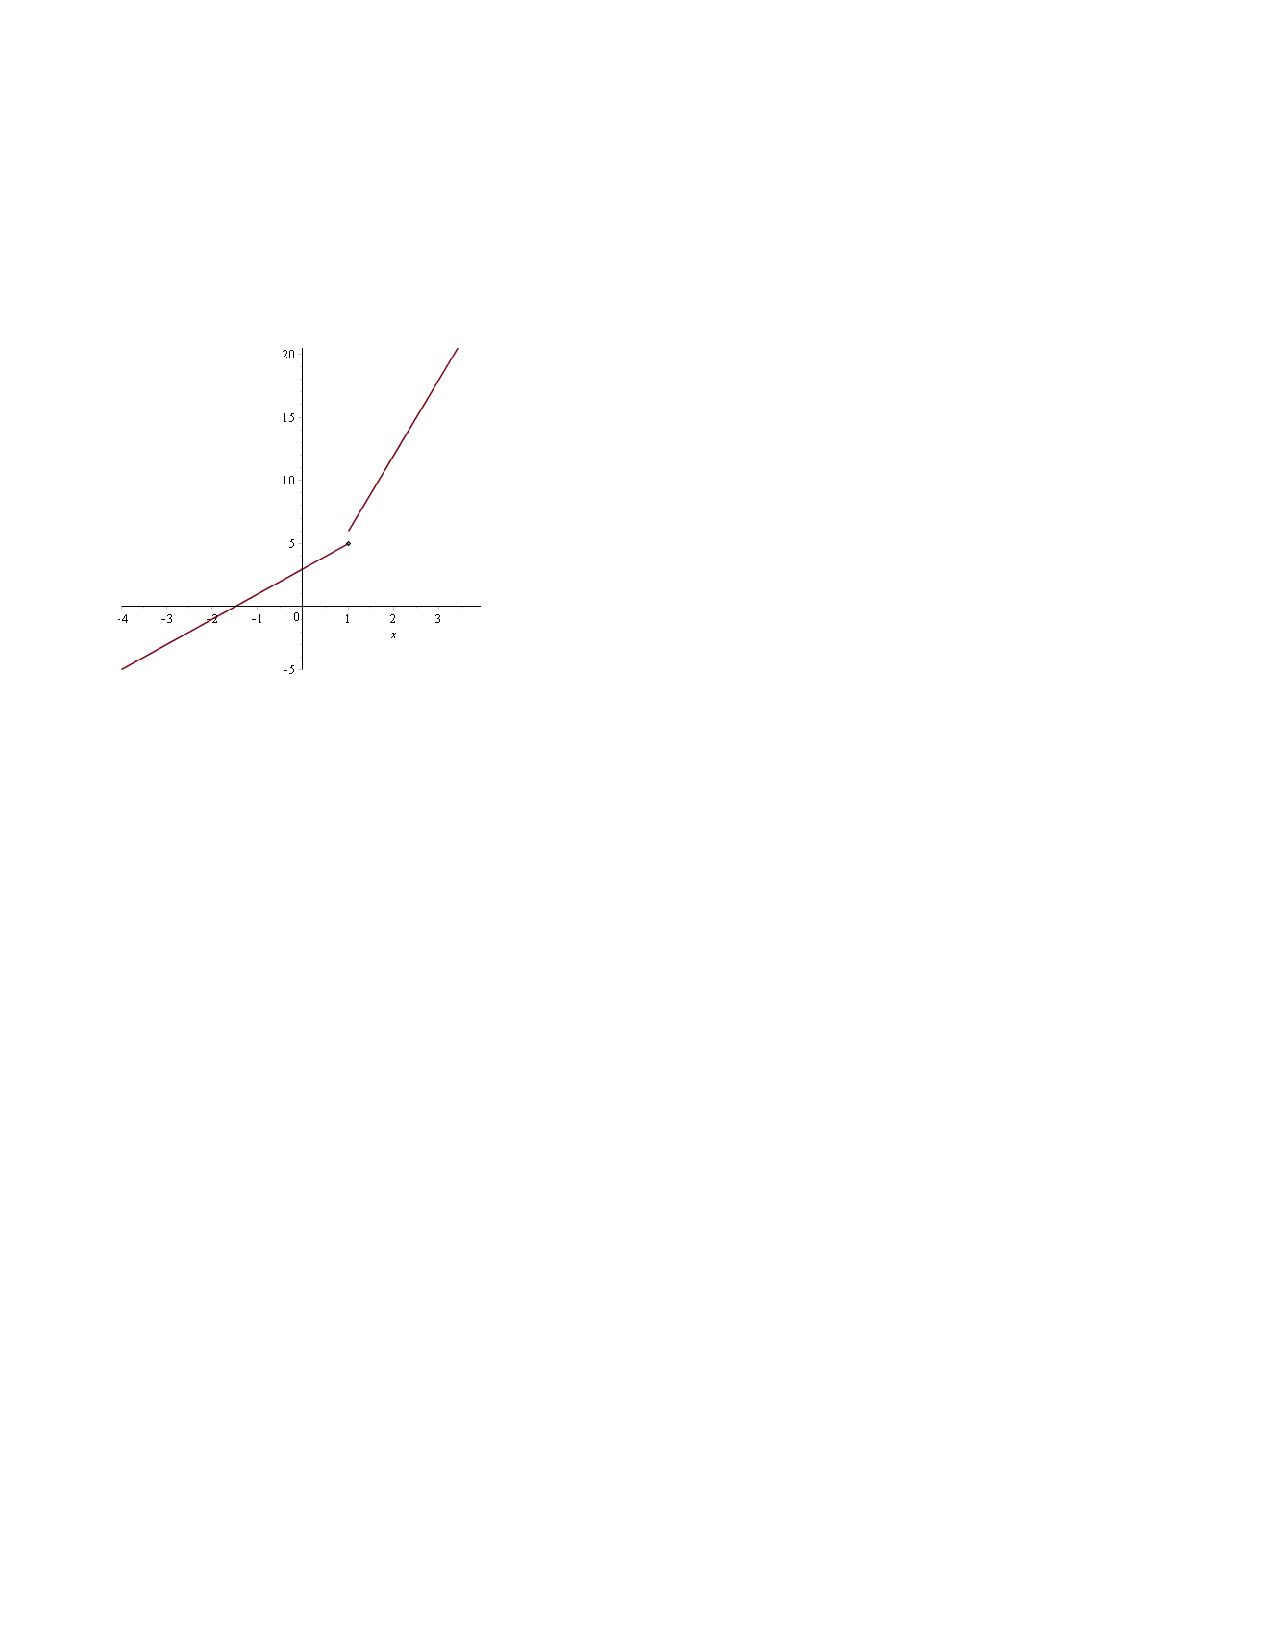
\includegraphics[trim= 640 500 250 210]{Images/Figure6.pdf}
	\end{image}
      \end{freeResponse}

    \item  What are you trying to maximize or minimize?
      Write an equation for it in terms of the variables from (a).
      \begin{freeResponse}
        We want to minimize the combined area of the garden and border.  If $A$ denotes this area, then an equation for $A$ is
        $$ A = (x+4)(y+2) $$
      \end{freeResponse}

    \item  What is your constraint?
      Write a constraint equation in terms of the variables from (a).
      \begin{freeResponse}
        We know that the area of the flower garden is $30 \, m^2$.  So our constraint equation is
        $$ xy = 30 $$
      \end{freeResponse}
      
    \item  Reduce your optimization equation to one variable using the constraint equation.

      \begin{freeResponse}
        $$ x = \frac{30}{y} \quad (\text{Note that } y \neq 0) $$
        \begin{align}
          A &= \left( \frac{30}{y} + 4 \right)(y+2) \\
            &= 30 + 4y + \frac{60}{y} + 8 \\
            &=4y + \frac{60}{y} + 38 \label{eqn3}
        \end{align}
      \end{freeResponse}
		
    \item  What is the interval on which your variable makes sense?
      Is it open or closed?
      What does this mean for the method of finding the absolute max or min?
      \begin{freeResponse}
        $0 < y < \infty$, which is an open interval.
        So we need there to only be one critical point to equation \eqref{eqn3} in the domain of $y$, and then we need to show that this critical point is a local minimum.
        This will imply that the critical point is an absolute minimum (since there is only one critical point).  
      \end{freeResponse}
		
    \item  Use the appropriate method to find and justify your absolute extremum.
      \begin{freeResponse}
        We need to differentiate equation \eqref{eqn3} with respect to $y$, set this derivative equal to $0$, and then solve:
        $$ \dd[A]{y} = 4 - \frac{60}{y^2} :=0 $$
        $$ \frac{60}{y^2} = 4 $$
        $$ 4y^2 = 60 $$
        $$ y^2 = 15 $$
        $$ y = \pm \sqrt{15} $$
        Since $-\sqrt{15}$ is not in our domain, the only critical point of $A(y)$ in the interval $(0,\infty)$ is $\sqrt{15}$.  
        Thus, if $y=\sqrt{15}$ is a local minimum for $A$, then it will be an absolute minimum.  
        Using the $2^{nd}$ derivative test:
        $$ \dd[^2A]{y^2} = \frac{120}{y^3} $$
        $$ \eval{\dd[^2A]{y^2}}_{y=\sqrt{15}} = \frac{120}{15 \sqrt{15}} > 0. $$
        
        Since $A(y)$ is concave up at $y=\sqrt{15}$, this point is a local (and thus, absolute) minimum of $A(y)$.  
        Note that we also could have used the first derivative test to show that $y=\sqrt{15}$ was a local minimum of $A$.
      \end{freeResponse}
      
    \item  Be sure to answer the question asked in the original problem.
      \begin{freeResponse}
        Since $y=\sqrt{15} \, m$, we have that
        $$ x = \frac{30}{y} = \frac{30}{\sqrt{15}} = \frac{30 \sqrt{15}}{15} = 2 \sqrt{15} \, m $$
      \end{freeResponse}
    \end{enumerate}
\end{problem}

%problem 6
\begin{problem}
  What point on the parabola $y=5-x^2$ is closest to the point $(4,7)$?
  \begin{freeResponse}
    \begin{image}
      \includegraphics[scale = 0.3]{Images/"distance to parabola".png}
    \end{image}

    We have ``to minimize $d \iff$ to minimize $d^2$''.

    Objective function:
    \begin{align*}
      d^2 = (x-4)^2 + (y-7)^2 \mbox{ and } y = 5 - x^2 &\implies d^2 = (x-4)^2 + \left((5 - x^2) -7 \right)^2\\
      &\implies f(x) = (x-4)^2 + (x^2 + 2)^2
    \end{align*}
    We may assume $\mbox{Domain}(f) = [0, \sqrt{5}]$.

    Critical points:
    \begin{align*}
      f'(x) &= 2(x-4) + 2(x^2 + 2) \cdot 2x\\
      &= 4x^3 + 10x - 8.
    \end{align*}
    $f'$ is defined everywhere on $(0, \sqrt{5}) \implies$ critical points only occur where $f'(x) = 0$:
    \begin{align*}
      f'(x) = 0 &\iff 4x^3 + 10x - 8 = 0\\
     \text{using a calculator to find an approximate value of}\ x &\implies x \approx 0.67628 
    \end{align*}

    Find absolute minimum:
    \begin{align*}
      f(0) &= 20\\
      f(0.67628) &\approx 17.1\\
      f(\sqrt{5}) &\approx 52.1\\
      &\implies \mbox{absolute minimum at $x \approx 0.67628$}
    \end{align*}
  \end{freeResponse}
\end{problem}

%problem 7
\begin{problem}
  A rectangle is constructed with one side on the positive $x$-axis, one side on the positive $y$-axis, and the vertex opposite the origin on the line $y=10-2x$.
  What dimensions maximize the area of the rectangle?
  What is the maximum area?
  \begin{freeResponse}
    The four vertices of the rectangle are $(0, 0)$, $(x, 0)$, $(x, y)$, and $(0, y)$:
    \begin{center}
      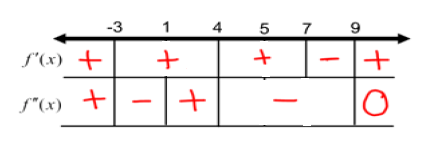
\includegraphics[scale = .5]{Images/figure8.png}
    \end{center}
    We're trying to maximize the area $A = x \cdot y$.

    First, we want to turn this area formula into a function of $x$.
    To do that we use the constraint $y = 10 - 2x$.
    Substituting, we find the function we're trying to maximize is $A(x) = x (10 - 2x) = 10x - 2x^2$.

    Next, we need to identify the domain of $A$.
    The smallest $x$ can be, to give a nonnegative area, is $x = 0$.
    To find the largest value we compute the $x$-intercept of $y = 10 - 2x$:
    \begin{align*}
      10 - 2x = 0 &\implies x = 5.
    \end{align*}
    Therefore $\mathrm{Domain}(A) = [0, 5]$.

    Next we locate the critical points of $A$.
    Since $A'(x) = 10 - 4x$ is defined on all the interior points of $[0, 5]$, to locate critical points solve 
    \begin{align*}
      A'(x) = 0 &\iff 10 - 4x = 0\\
                &\iff x = \frac{5}{2}.
    \end{align*}

    To finish we evaluate $A$ at $0$, $5/2$, and $5$:
    \begin{align*}
      A(0) &= 0\\
      A(5/2) &= 25/2\\
      A(5) &= 0
    \end{align*}

    Therefore the maximum area occurs when the rectangle has a base with length $5/2$ units and height with length of $5$ units.
    The area with these dimensions is $25/2$.
  \end{freeResponse}
\end{problem}
\end{document} 
